\section{First limit extraction}
\label{sec:firstExtraction}
% ---- ---- ---- ---- ---- ---- ---- ---- ---- ---- ---- ---- ---- ---- ---- ---- ---- ---- ---- ---- ---- ---- ----

\subsection{Event selection and limit extraction technique}
% .... .... .... .... .... .... .... .... .... .... .... .... .... .... .... .... .... .... .... .... .... .... ....

We extract a first limit for the Standard Model Higgs boson after applying few additional cuts on
top of the preselections. The detailed description of this limit extraction can be found in a
dedicated Analysis Note \cite{CMS-AN-12-029}.

Events are selected with single lepton triggers throughout the whole data taking, as detailed in
Table~\ref{tab:HLT}. 

The two jets with the highest transverse momentum are chosen as the candidates of the W decay, and
only events where they are compatible with the W mass are selected ($65\GeVcc < m_{jj} < 95\GeVcc$).\\
To further enhance the signal over background ratio, we exploit the fact that Higgs decay products 
tend to be emitted in the central part of the detector, at variance with the behaviour of the W+jets
background. We therefore require events to have the lepton in the barrel ($|\eta|<1.5$), and the two
jets to be closer than 1.5 in $\eta$. Besides, the $|\eta|$ of the di-jet system is required to be
smaller than 3.\\
Finally, the cut on the MET and on the leptonic W transverse mass are set to 30~GeV. 

\begin{table}[htb]
 \begin{center}

%%   \scalebox{0.85}{
   \subfloat[Trigger paths for electrons.
   \label{tab:electronHLT}]{
   \begin{tabular}{c|c|c|l}
     \hline
     period & run range & dataset name & trigger path name                                                                                               \\
     \hline
     (e-i) & 190456 - 191930 & \texttt{Run2012A-PromptReco-v1} & \texttt{HLT\_Ele27\_WP80\_v*}   \\
     (e-ii) & 193829 - 195775 & \texttt{Run2012B-PromptReco-v1} & \texttt{HLT\_Ele27\_WP80\_v*}  \\
     \hline
   \end{tabular}}
%%   }

   \vskip 1cm

%%   \scalebox{0.85}{
   \subfloat[Trigger paths for muons\label{tab:muonHLT}]{
   \begin{tabular}{c|c|c|l}
      \hline
      period & run range & dataset name & trigger path name                     \\
                  \hline \hline
      ($\mu$-i) & 190456 - 191930 & \texttt{Run2012A-PromptReco-v1} & \texttt{HLT\_IsoMu24\_eta2p1\_v*}     \\
      ($\mu$-ii) & 193829 - 195775 & \texttt{Run2012B-PromptReco-v1} & \texttt{HLT\_IsoMu24\_eta2p1\_v*}     \\
      \hline
   \end{tabular}}
%%   }

 \end{center}
 \caption{List of trigger paths used to select events for this analysis, in the final state with
 electrons (a) and with muons (b).}
 \label{tab:HLT}
\end{table}

For each mass hypothesis, the limit on the Standard Model Higgs cross section is obtained from a fit
of the four-body invariant mass spectrum, as the place where the appearance of a Higgs resonance
is expected. The mass fit with a background-only hypothesis and a signal-plus-background hypothesis
to extract the exclusion C.L. is performed within the CMS Combination Tool.

The signal hypothesis is described by a fit on the Monte Carlo invariant mass shape performed for
each mass hypothesis independently. Figure~\ref{fig:signalShape} shows two examples of such fit.

\begin{figure}[htb]
\begin{center}
  \subfigure[]{
  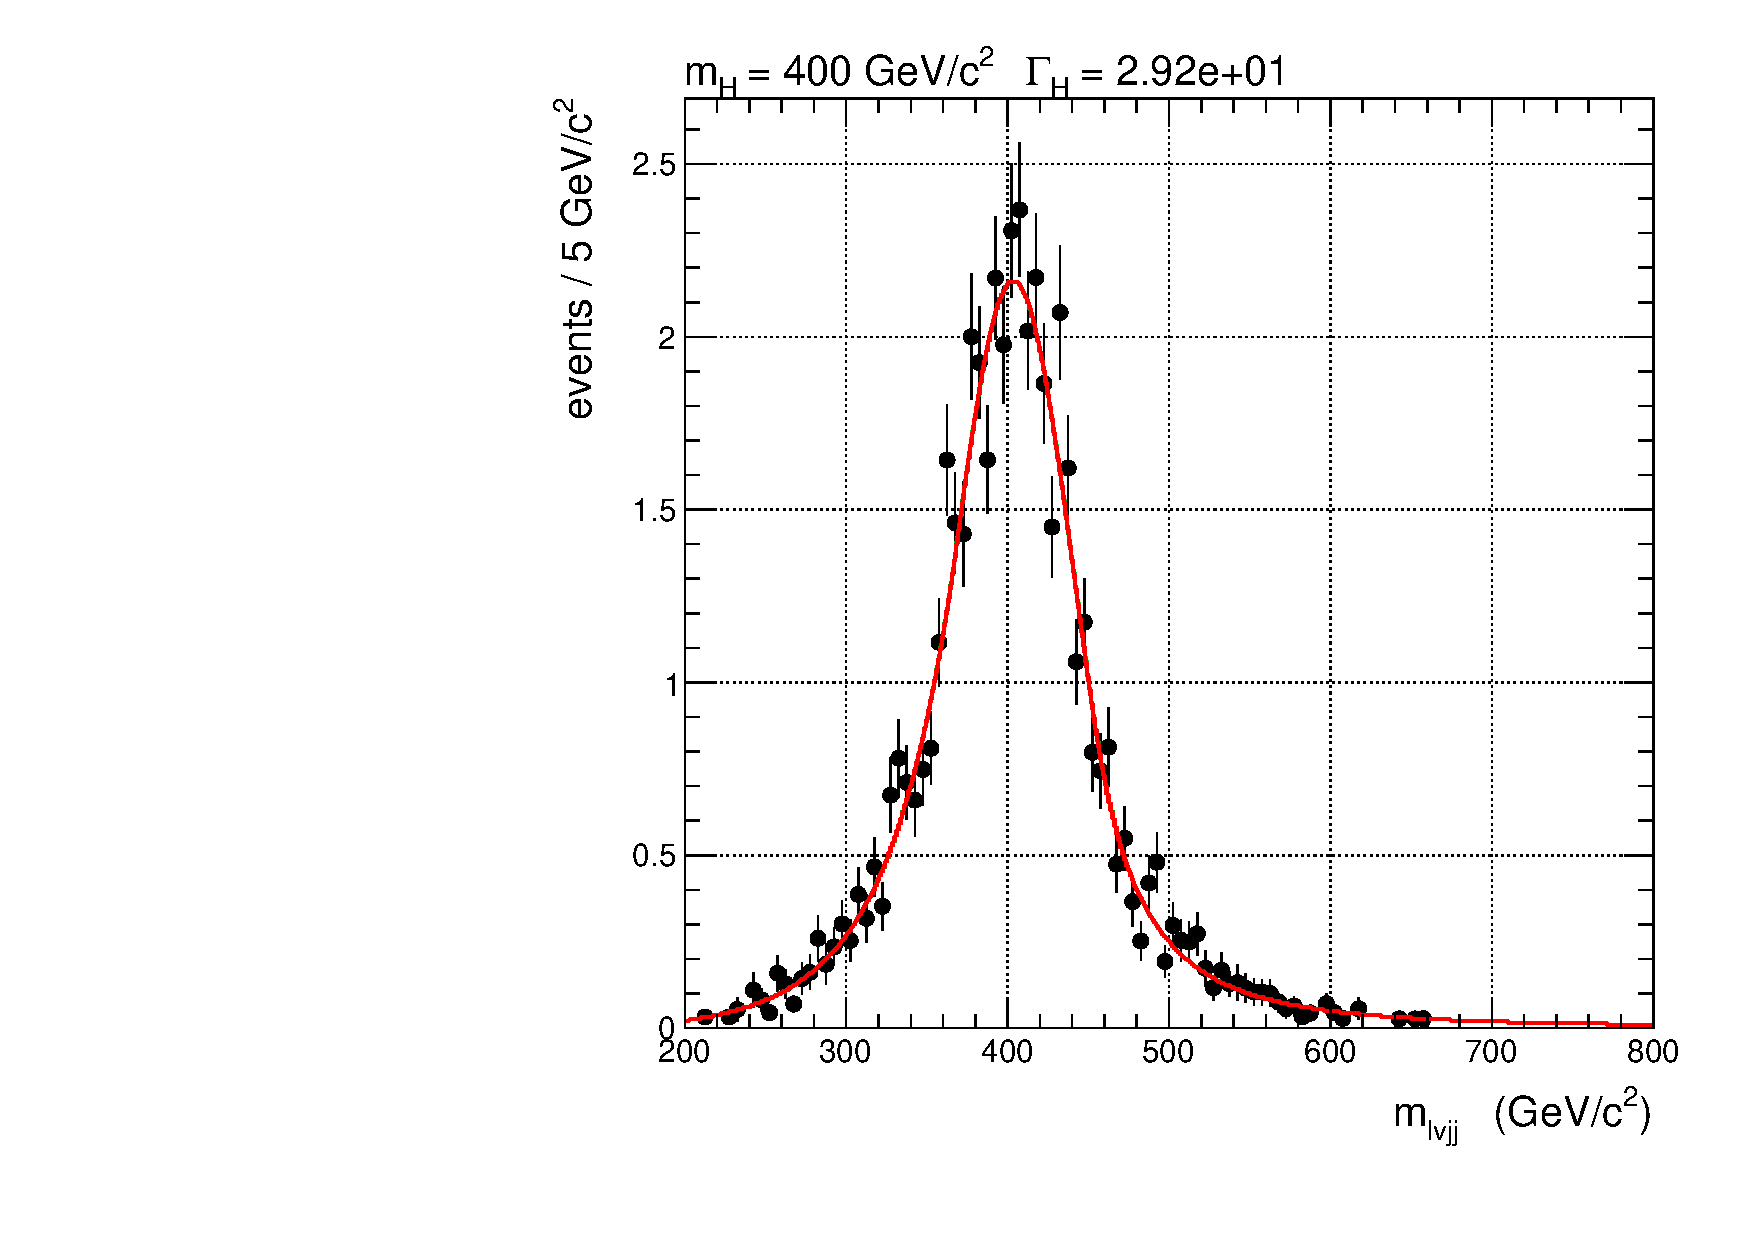
\includegraphics[width=0.45\textwidth]{plots/limitplot/signalShape_MH400.pdf}}
  \subfigure[]{
  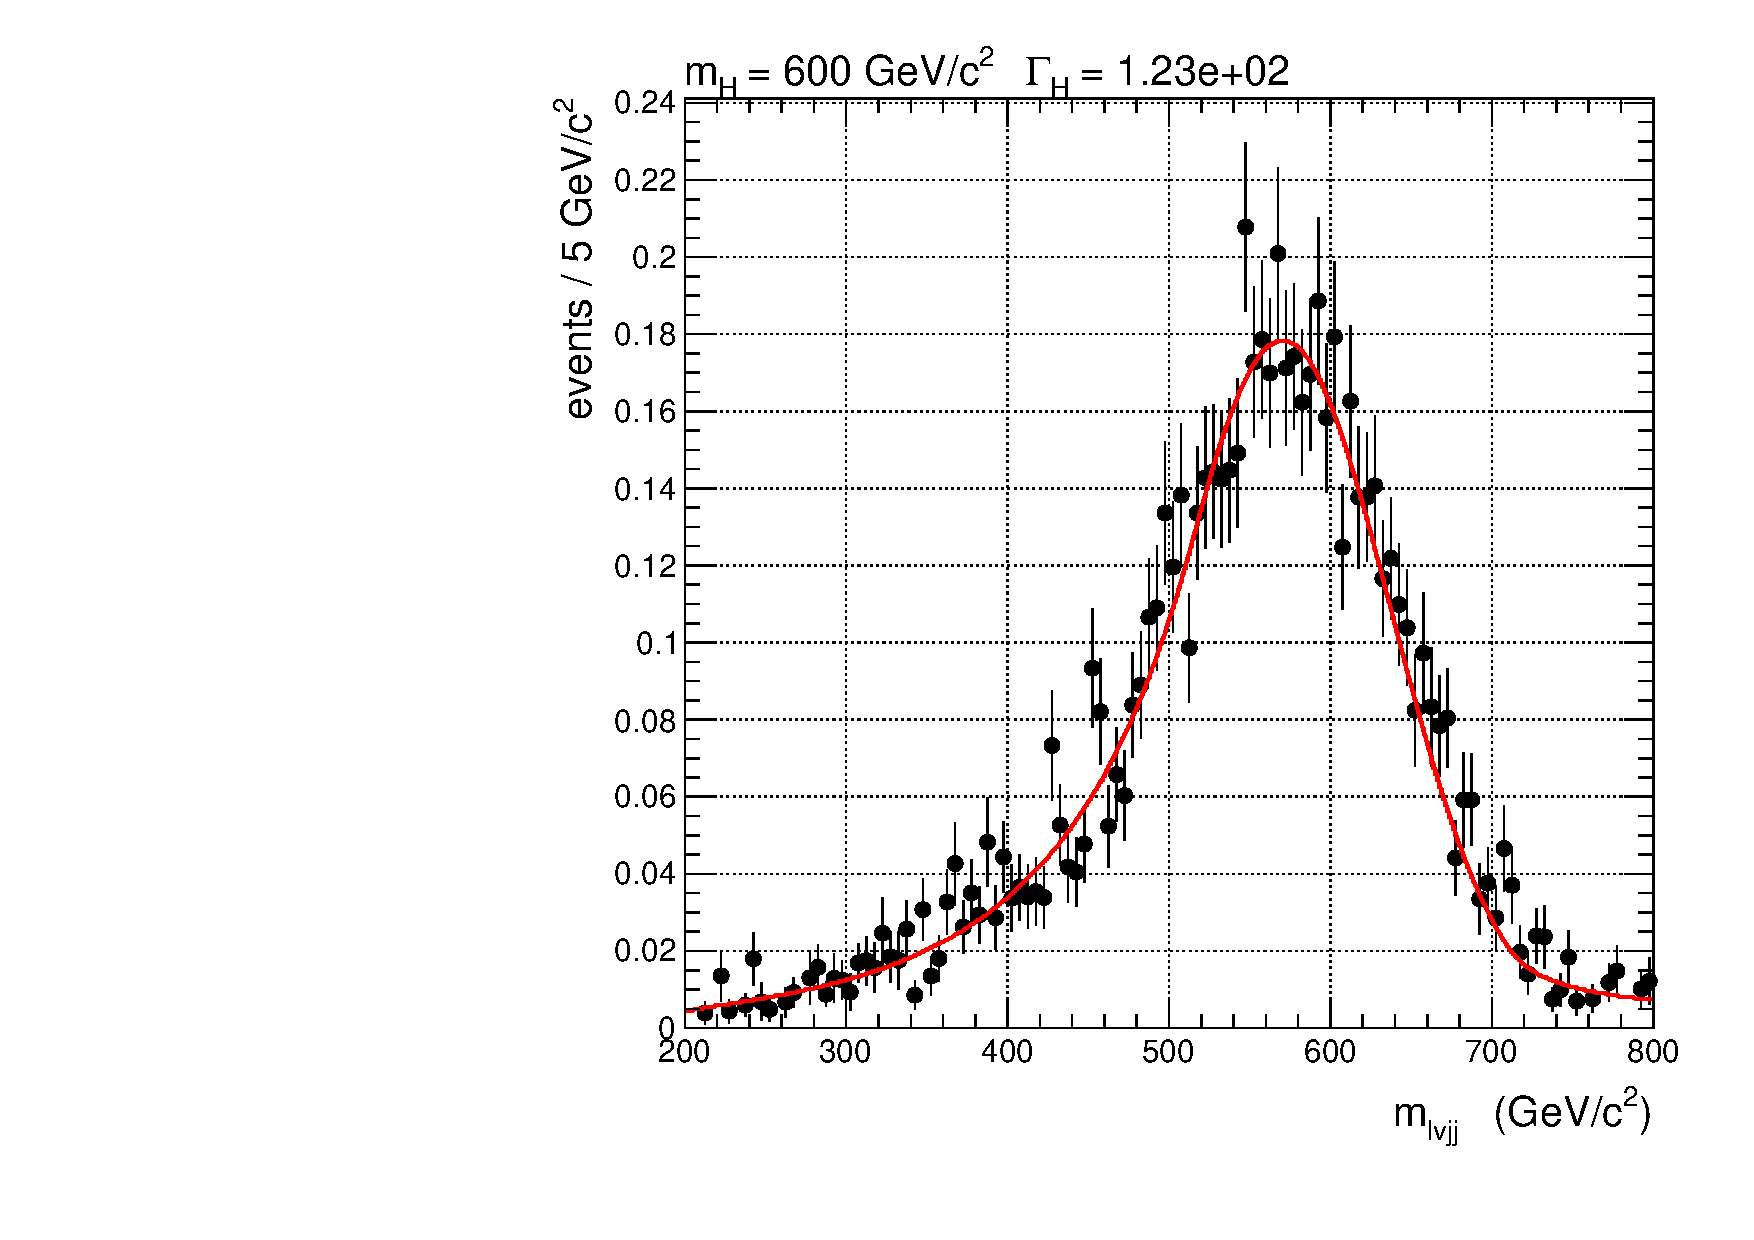
\includegraphics[width=0.45\textwidth]{plots/limitplot/signalShape_MH600.pdf}}
  \caption{Higgs boson invariant mass shape, as obtained from a (a) 400\GeVcc and (b) 600\GeVcc
           simulation. All the proper weighting factors taken into account. The fit function is
           constituted by a gaussian core smoothly joined to a high-mass and a low-mass power law
           tail. This smooth function is used as signal input for the  the limit extraction.}
  \label{fig:signalShape}
\end{center}
\end{figure}

To choose the best shape for the background we performed a dedicated study. We identified four
functional families, intended to span the possibilities of the true distribution to which
signal-free data would tend if we disposed of a nearly infinite statistics. The functional forms are:
polynomials ($\mathcal{T}(x;\mu,kT) \times \sum a_i x^i $), exponentials
($\mathcal{T}(x;\mu,kT) \times \sum N_i e^{-\lambda_i x}$), exponentiated polynomials
($\mathcal{T}(x;\mu,kT) \times e^{\sum a_i x^i}$) and power laws
($\mathcal{T}(x;\mu,kT) \times \sum N_i (x-a_i)^{-n_i}$), where all functions are multiplied by
$\mathcal{T}(x;\mu,kT)$, a fermi function intended to model the low invariant-mass turn-on. The
order of the functional forms is chosen after a study of fits on the MC simulation: for each family,
the order order of the fit function is raised until the goodness of the fit significantly improves.
The result is that a third order exponentiated polynomial, a second order exponential,  and a first
order power law are kept as background model candidates. Since a very  large number of degrees of
freedom is needed for the polynomials to well reproduce the invariant mass shape, the whole family
is discarded.

Among the resulting background model candidates, the power law is chosen, being the one that
minimizes the number of degrees of freedom and the bias on the background estimation, as explained
in the following section. To summarize, the background-only hypothesis is parametrized with this
function:

\begin{equation}
f_{\textnormal{bkg}}(x) = \frac{1}{e^{-(x-\mu)/kT} + 1} \cdot N \bigg(\frac{500+a}{x+a}\bigg)^n~,
\label{eq:fit_bkgModel}
\end{equation}

where all parameters are free to float in the fit. 
Figure~\ref{fig:backgroundShape} shows the four-body mass distribution 
of the observed events after the preselections, 
in the sidebands of the $m_{jj}$ spectrum as the analysis is still blind, %FIXME after unblinding
overlapped to a fit of the chosen background-only shape, 
performed outside the combination tool for illustrative purposes.

\begin{figure}[htb]
\begin{center}
 \subfigure[\label{fig:backgroundShape_mu}]{
  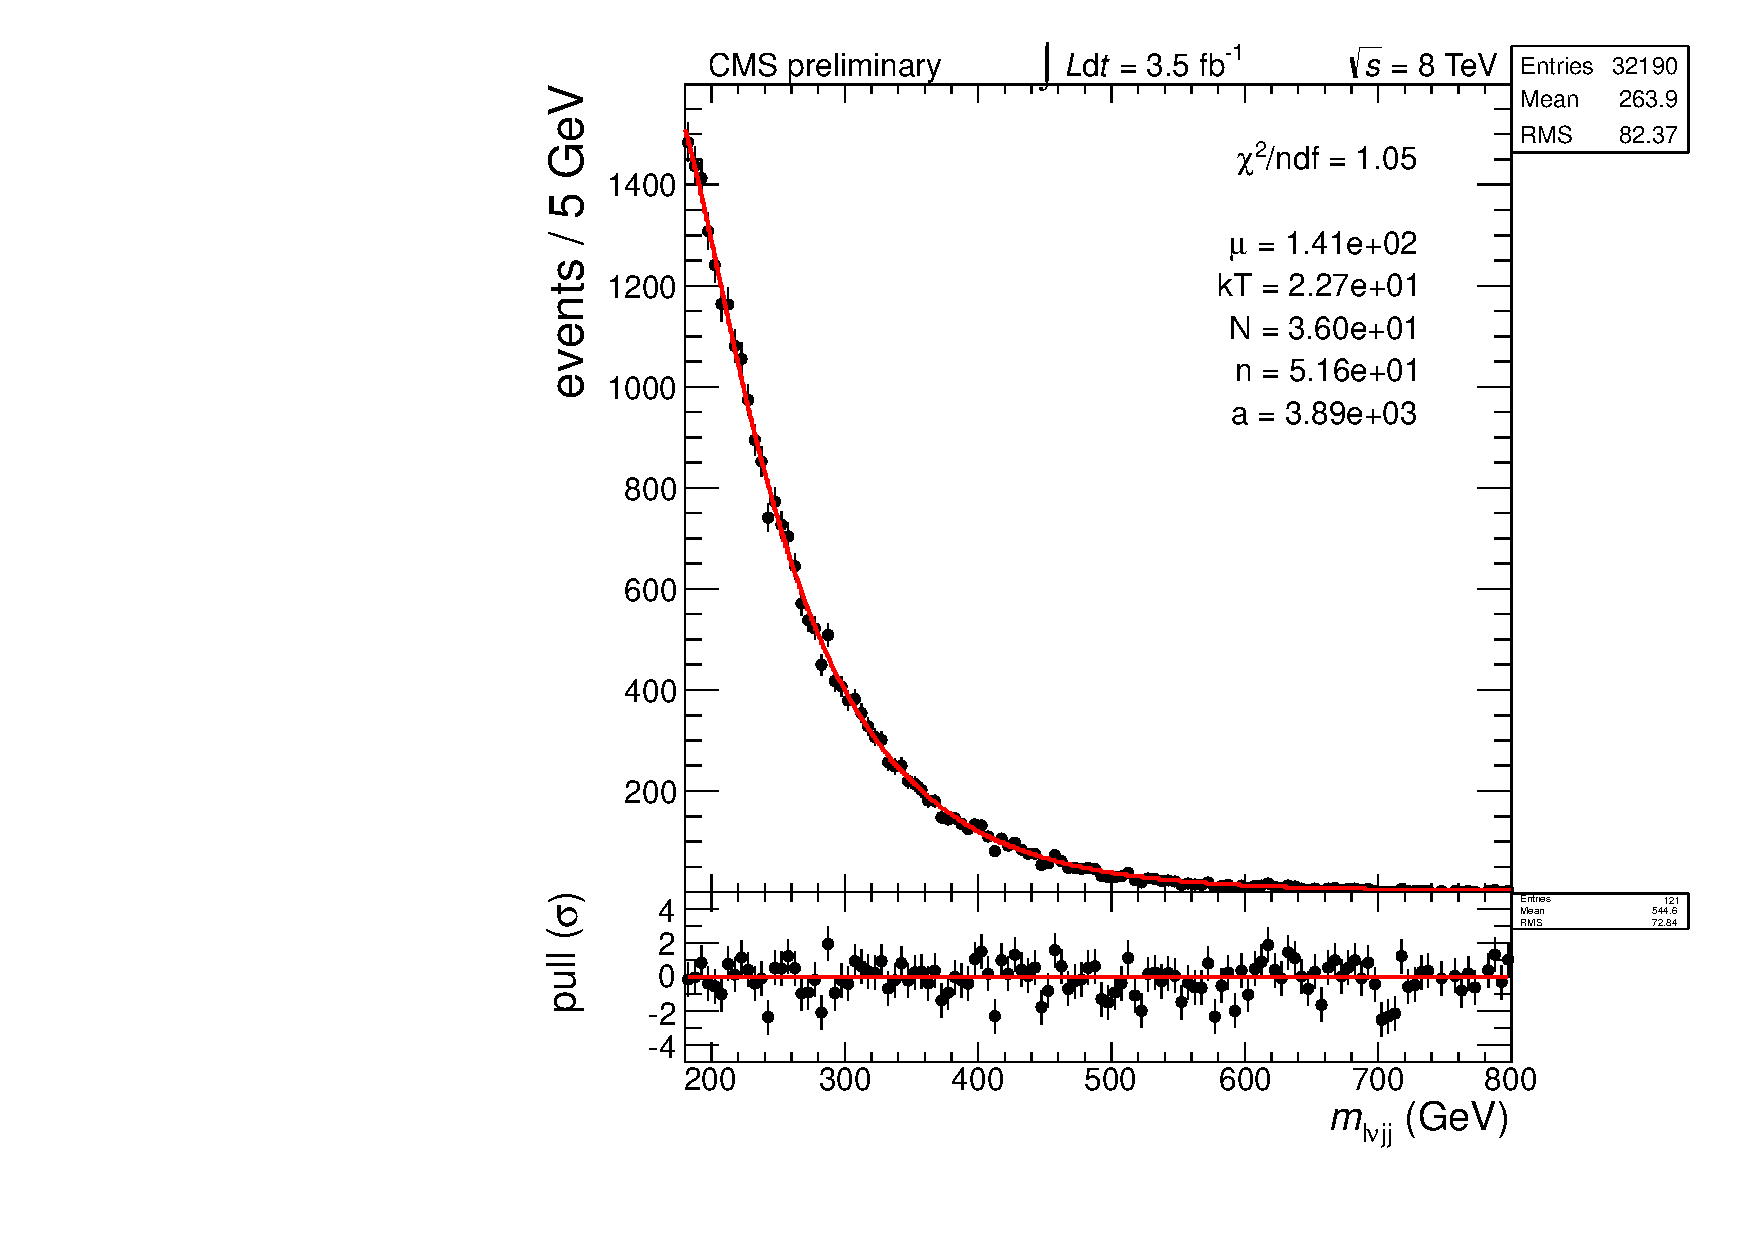
\includegraphics[width=0.49\textwidth]{plots/lin_data_mu_attenuatedPowerLaw_lepNuW_m_KF.pdf}
  }
 \subfigure[\label{fig:backgroundShape_e}]{
  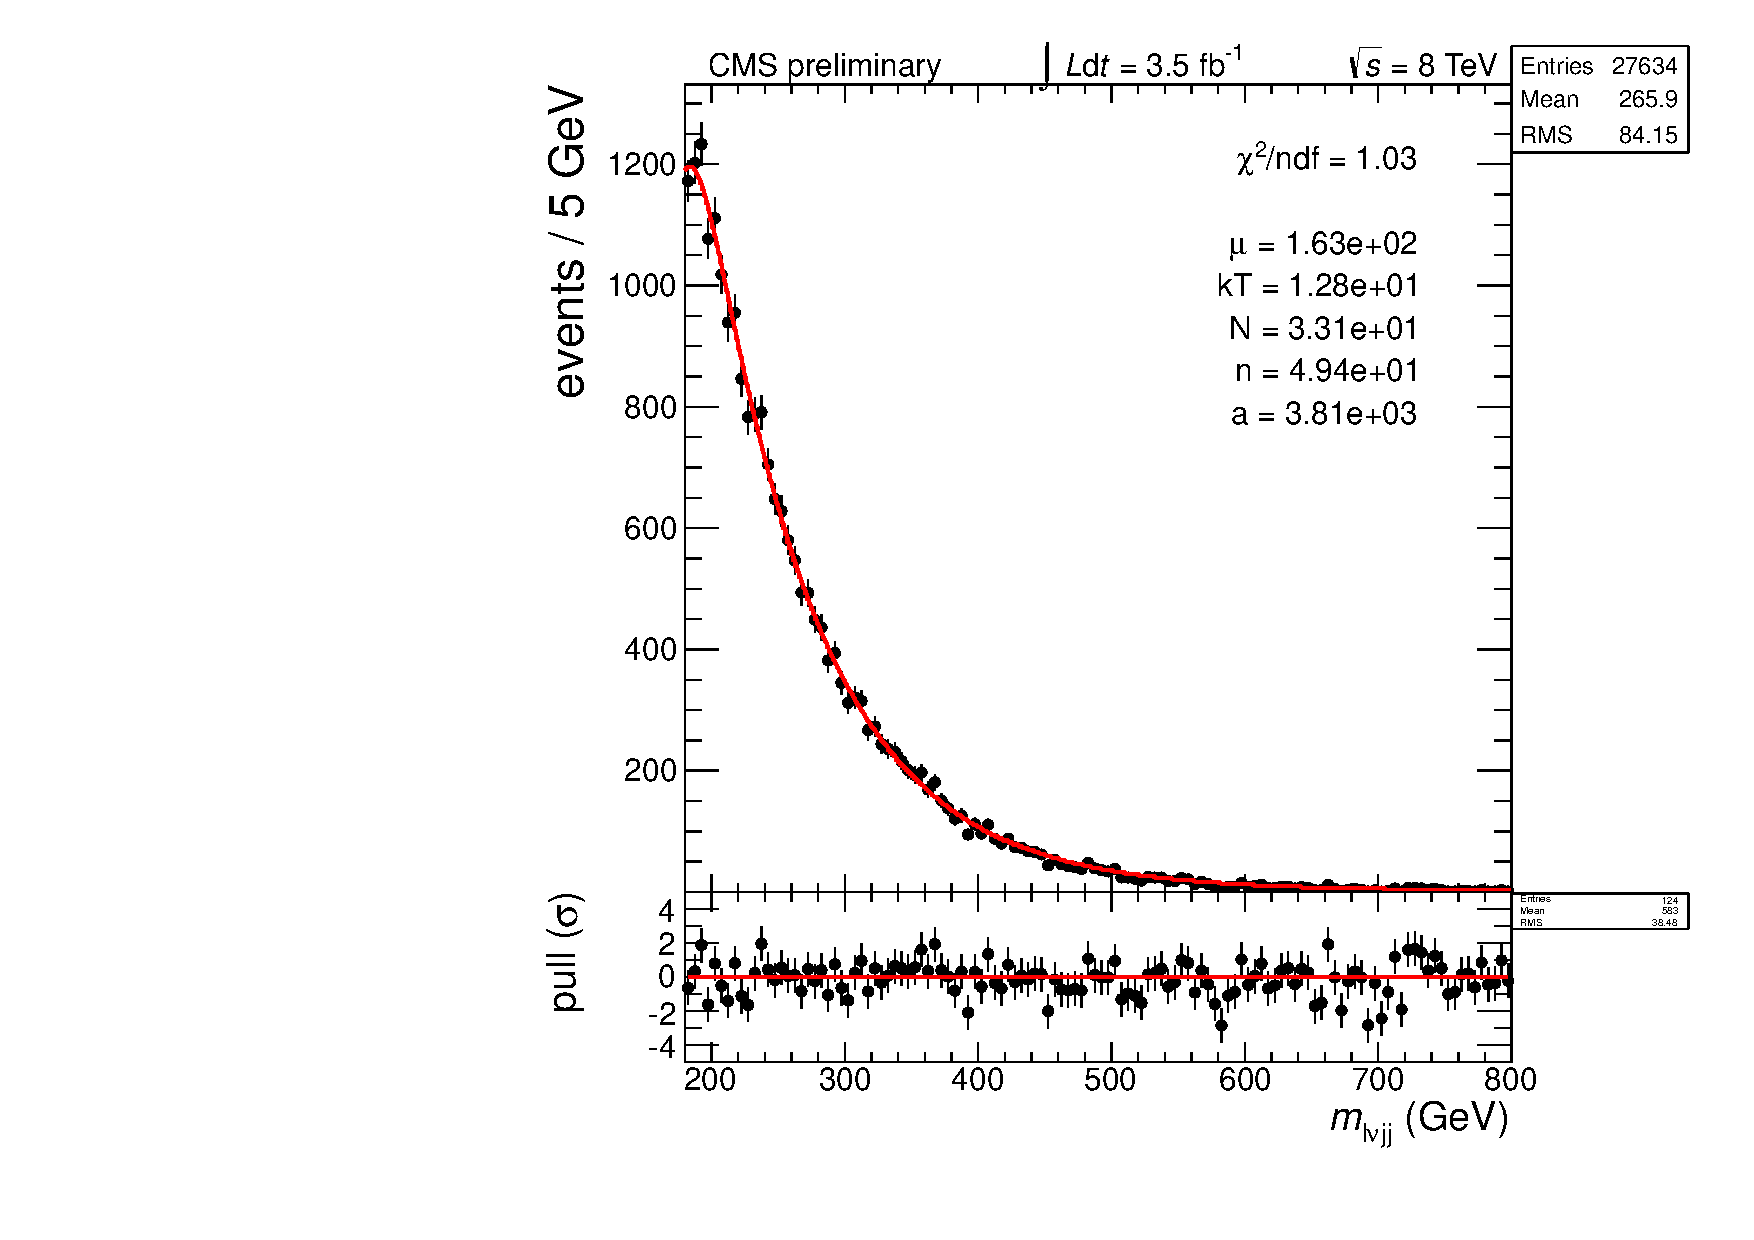
\includegraphics[width=0.49\textwidth]{plots/lin_data_e_attenuatedPowerLaw_lepNuW_m_KF.pdf}
  }

  \caption{The four-body mass distribution of the observed events after preselections, for
          muons (a) and electrons (b), with a fit of the background-only shape
          superimposed. The fit is performed outside the combination
          tool for illustrative purposes.
          The fit is performed in the sidebands of the $m_{jj}$ spectrum as the analysis is still blind.%FIXME after unblinding
          }
  \label{fig:backgroundShape}
\end{center}
\end{figure}



\subsection{Uncertainties on the background evaluation}
% .... .... .... .... .... .... .... .... .... .... .... .... .... .... .... .... .... .... .... .... .... .... ....

The statistical uncertainty on the background is derived within the limit calculation from the
uncertainties on the parameters determination in the fit. Additionally, a systematic uncertainty
related to the choice of the specific background model of Equation~\ref{eq:fit_bkgModel} is
accounted for. The set of functions used to estimate the bias was defined in the previous section,
and consists of
$$
\mathcal{S} = \{\textnormal{attExp2,attPL1,attExpPol3}\}~,
$$
where we have:
\begin{equation}
\begin{split}
\textnormal{attExpPol3} & \doteq \mathcal{T}(x;\mu,kT) \times N e^{a_1 x + a_2 x^2 + a_3 x^3} \\
\textnormal{attExp2}    & \doteq \mathcal{T}(x;\mu,kT) \times N_1 \left( e^{-\lambda_1 x} + N_2 e^{-\lambda_2 x} \right) \\
\textnormal{attPL1}     & \doteq \mathcal{T}(x;\mu,kT) \times N \left(\frac{500+a}{x+a}\right)^n
\end{split}
\quad{.}
\end{equation}

To estimate the bias introduced by choosing one of the above functions to fit the mass spectra, the
following procedure has been followed:

\begin{itemize}
\item choose one of the functions above and use it as parent distribution $P(x)$;
\item generate a toy dataset according to $P(x)$ and corresponding to a large amount of accumulated
statistics (equivalent to $\sim 10000\fbinv$). The parameters of $P(x)$ are determined with a fit on
data\footnote{The data sample was preferred to the MC for the determination of the parameters of
the parent functions since the MC statistics is significantly lower than the data, and this can lead
to an artificially larger bias estimation.};
\item fit each toy dataset with all the test fit function $F(x)$ from the list above and and, for
each Higgs mass window $[x_{\textnormal{low}},x_{\textnormal{high}}]$, compute
$\delta(n_B)_{FP} = n_B^{\textnormal{fit}} - n_B^{\textnormal{parent}}$, where
$n_B^{\textnormal{fit}} = \int_{x_{\textnormal{low}}}^{x_{\textnormal{high}}} F(x) dx$ and
$n_B^{\textnormal{parent}} = \int_{x_{\textnormal{low}}}^{x_{\textnormal{high}}} P(x) dx$
\item iterate the procedure for all $P(x)$ in $\mathcal{S}$.
\end{itemize}
In the end, for each combination of a test fit function $F_i(x)$ and a parent function $P_j(x)$,
a value of $\delta(n_B)_{ij}$ is obtained for each of the 8 different Higgs mass hypotheses (the
indices $i$ and $j$ can run on the set of functions $\mathcal{S}$). The distribution of
$\delta(n_B)_{ij}$ obtained when varying the parent function $P(x)$ gives a quantitative
indication of the bias introduced by choosing a given $F(x)$ as the background fit model.

In fact, the bias due to possible difference in shape between the model and data corresponds to
fake signals and dips in the invariant mass spectrum that would systematically affect the
determination of an hypothetical Higgs signal. Therefore, the bias originating from the choice of a
specific background shape is introduced as an additional systematics on the signal, quoting it as a
fraction with respect to the total number of expected signal events. Table~\ref{tab:attPL_bias}
shows the obtained values as a function of the Higgs mass hypothesis.

\begin{table}[h!t]
 \begin{center}
   \begin{tabular}{c|c|c|c}
     \hline
     \multicolumn{2}{c|}{\small{$e\nu{}jj$}} &
     \multicolumn{2}{c} {\small{$\mu{}\nu{}jj$}} \\
     $m_{\textnormal{H}}$ &  unc. & $m_{\textnormal{H}}$ &  unc. \\
     \hline
     \hline
     250 & 54.8\%   &   250 &  9.1\% \\
     300 & 27.2\%   &   300 & 10.9\% \\
     350 & 28.3\%   &   350 & 11.6\% \\
     400 & 29.2\%   &   400 & 12.3\% \\
     450 & 21.8\%   &   400 &  3.7\% \\
     450 &  5.5\%   &   450 & 21.6\% \\
     550 & 38.5\%   &   500 & 41.2\% \\
     600 & 71.6\%   &   550 & 60.8\% \\
     \hline
   \end{tabular}
 \end{center}
 \caption{Signal uncertainty due to the background shape systematic for electron (left) and muon
         (right) final states.}
 \label{tab:attPL_bias}
\end{table}



\subsection{Uncertainties on the signal evaluation}
% .... .... .... .... .... .... .... .... .... .... .... .... .... .... .... .... .... .... .... .... .... .... ....

The sources of systematics on the signal considered in this case are the following:
\begin{itemize}
\item the luminosity uncertainty is considered 2.2\%;
\item the jet energy scale is taken into account by coherently varying all the jets with $\pt>15~\GeV$
      within the error provided by the CMS measurements, and the effect of such a variation is
      considered in the MET. The unclustered MET is conservatively varied by 5\% in a fully
      correlated fashion;
\item the uncertainty on pile-up comes from the limited knowledge of the number of pile-up events in
      data, quoted to be 5\%~\cite{PUScaling};
\item the uncertainty on the theoretical inclusive cross-section is taken from the LHC Cross Section
      Working Group calculations~\cite{LHCHiggsCrossSectionWorkingGroup:2011ti}, and the effects of
      pdfs on the acceptances are calculated according to the recipe provided by the same group;
\item the uncertainty on the Higgs mass shape is considered according the LHC Cross Section Working
      Group recommendations;
\item the uncertainty on the background shape modeling ranges from 2\% to 40\% on the signal rate;
\item trigger and lepton reconstruction efficiencies or scale factors are propagated through the
      analysis according to their measurements uncertainties;
\item the b-tagging uncertainty is propagated in the analysis chain, for the three-jets bin, by using
      the prescriptions from the b-POG and found to be less than a percent over the full mass range.
\end{itemize}
Table~\ref{tab:fitSystematics} summarizes all the sources of uncertainty considered, with the
typical effect on the signal.

\begin{table}[h!]
\begin{center}
\begin{tabular}{l|c}
\hline
source of uncertainty &  impact on signal  \\
\hline
\hline
background modeling                        &  4-70\% \\
Higgs line-shape                           & 10-30\% \\
cross-section                              & 15-20\% \\
luminosity                                 &   2.2\% \\
jet energy scale and MET                   &   2-3\% \\
theo acceptances (pdf)                     &   1-2\% \\
lepton trigger efficiency                  &  $<$1\% \\
lepton efficiency                          &   1-2\% \\
pile-up                                    &  $<$1\% \\
b-tag veto                                 &  $<$1\% \\
\hline
\end{tabular}
\end{center}
\caption{Sources of systematics considered in the fit analysis, with the corresponding value.}
\label{tab:fitSystematics}
\end{table}



\subsection{The obtained limit}
% .... .... .... .... .... .... .... .... .... .... .... .... .... .... .... .... .... .... .... .... .... .... ....

The obtained limit,
with the CLs method, is reported in Figure~\ref{fig:firstLimit}.
To compute the limit value in the mass points where the MC simulation is not available
signal shapes and systematics are interpolated.\\

\begin{figure}[htb]
\begin{center}
   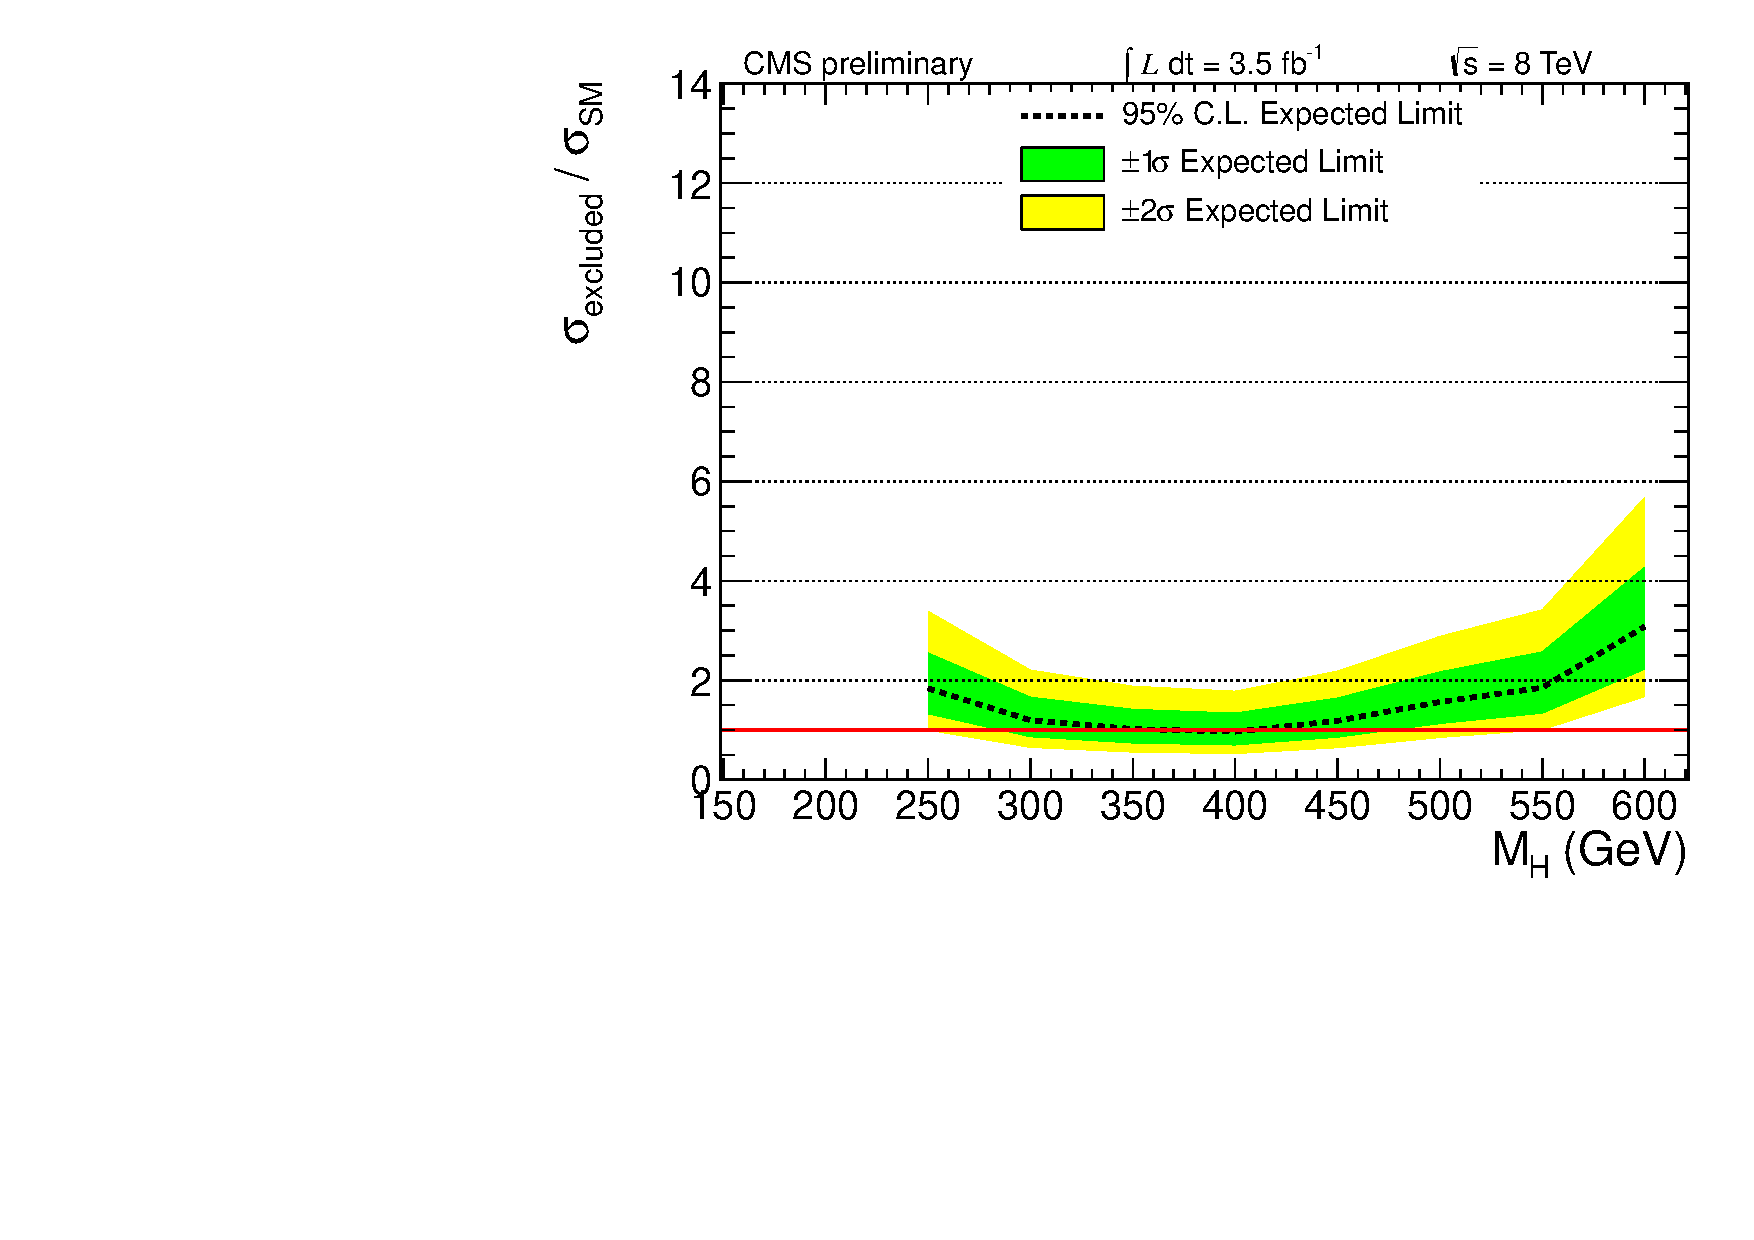
\includegraphics[width=0.6\textwidth]{plots/limitplot/limit_first.pdf}
   \caption{The Standard Model Higgs exclusion limit, obtained by a shape fit just after the preselections.}
 \label{fig:firstLimit}
\end{center}
\end{figure}

The observed 95\% confidence level exclusion limit for the SM Higgs boson production is in the mass range $XXX-YYY\GeV$.

To improve this limit, a tighter selection scheme has been designed, aimed at increasing the
signal-over-background ratio after the selections, together with a full set of data driven
background evaluations.
